\documentclass[final,3p,times,number]{elsarticle}
\usepackage[utf8]{inputenc}
\usepackage{graphicx}
\usepackage{booktabs}
\usepackage{array}
\usepackage{tabularx}
\usepackage{amsmath}
\usepackage{amssymb}
\usepackage{placeins}
\usepackage{float}
\usepackage[font=small,skip=6pt]{caption}
\usepackage{microtype}
\usepackage{tikz}
\usepackage{url}
\usetikzlibrary{arrows.meta,positioning,shapes.geometric}
\urlstyle{same}
\captionsetup{labelfont=bf,justification=centering}
\emergencystretch=2em
\newcolumntype{Y}{>{\raggedright\arraybackslash}X}
\setlength{\textfloatsep}{6pt plus 1pt minus 2pt}
\setlength{\floatsep}{6pt plus 1pt minus 2pt}
\setlength{\intextsep}{6pt plus 1pt minus 2pt}
\renewcommand{\arraystretch}{1.08}
\raggedbottom
\setcounter{topnumber}{5}
\setcounter{bottomnumber}{2}
\setcounter{totalnumber}{6}
\renewcommand{\topfraction}{0.95}
\renewcommand{\bottomfraction}{0.85}
\renewcommand{\textfraction}{0.05}
\renewcommand{\floatpagefraction}{0.85}
\journal{Engineering Applications of Artificial Intelligence}


\begin{document}
\begin{frontmatter}

\title{A Comprehensive Benchmark of 3D Segmentation Architectures for Brain Tumour Segmentation}

\author[vit]{Parth Mital\corref{cor1}}
\author[vit]{Ved Lawand}
\author[vit]{Biji C. L.}
\cortext[cor1]{Corresponding author. Email addresses: parth.mital2023@vitstudent.ac.in, ved.lawand2023@vitstudent.ac.in, biji.cl@vit.ac.in}

\affiliation[vit]{organization={School of Computer Science and Engineering, Vellore Institute of Technology},
city={Vellore},
country={India}}

\begin{abstract}
Brain tumour segmentation from multimodal magnetic resonance imaging (MRI) is important for diagnosis, treatment planning, and disease monitoring. This study benchmarks six three-dimensional segmentation architectures on the Brain Tumour Segmentation (BraTS) 2020 dataset: UNet, nnU-Net, VNet, UNETR, Swin UNETR, and TransBTS. All models are implemented in PyTorch with consistent preprocessing, data splits, training protocols, and evaluation metrics. Final test metrics are reported only for architectures whose notebooks contain captured final outputs; Swin UNETR is retained in the methodology but excluded from final comparison tables. UNet achieved the highest verified mean Dice score of 0.7999, followed by nnU-Net at 0.7945 and VNet at 0.7655. The results show that convolutional neural network (CNN) architectures remain highly competitive under the available training budget, while transformer-based models require longer schedules, pretraining, or larger datasets before their global context modelling can translate into stronger segmentation performance.
\end{abstract}

\begin{keyword}
Brain tumour segmentation, 3D UNet, Transformer, BraTS, Medical image analysis, Deep learning
\end{keyword}

\end{frontmatter}


\section{Introduction}

Gliomas are the most common and aggressive primary brain tumours, accounting for approximately 80\% of all malignant brain tumours worldwide \cite{ref5}. These tumours arise from glial cells and are classified into low-grade gliomas (LGG) and high-grade gliomas (HGG), with the latter being more invasive and associated with poorer patient outcomes. Accurate segmentation of these tumours from magnetic resonance imaging (MRI) scans is essential for several clinical tasks including diagnosis and grading, treatment planning, disease monitoring, and prognosis prediction. The BraTS challenge, established in 2012, has become the premier benchmark for evaluating brain tumour segmentation algorithms. It provides multimodal MRI scans consisting of four complementary sequences: T1-weighted (T1), T1-contrast-enhanced (T1CE), T2-weighted (T2), and fluid-attenuated inversion recovery (FLAIR). Alongside these scans, the dataset includes expert-annotated segmentation masks delineating three tumour sub-regions: whole tumour (WT), tumour core (TC), and enhancing tumour (ET) \cite{ref2}. The clinical significance of automated segmentation cannot be overstated. Manual delineation of brain tumours is time-consuming, requires specialised expertise, and suffers from inter-rater variability. Deep learning based segmentation methods have demonstrated the potential to automate this process, thereby reducing radiologist workload and providing consistent, reproducible results. However, the rapid proliferation of architectural innovations from convolutional neural networks to transformer based models has created a fragmented landscape where practitioners struggle to identify the most suitable approach for their specific clinical or research settings.

Despite significant advances in deep learning for medical image segmentation, several persistent challenges remain unaddressed in the existing literature. First, the proliferation of architectures from classic UNets to complex transformer hybrids creates confusion about which approach is optimal for clinical deployment. Researchers often introduce novel architectures without rigorous comparison against established baselines under controlled conditions, leading to inflated claims and unreliable benchmarks. Second, many published results use different preprocessing pipelines, training protocols, data splits, and evaluation metrics, making fair comparisons across studies difficult or impossible. A model that performs well under one set of conditions may fail under another, yet such nuances are rarely discussed. Third, transformer based models promise better global context modelling through self-attention mechanisms, but they require substantial computational resources, larger datasets, and careful hyperparameter tuning. This raises serious questions about their practical utility in resource-constrained clinical environments. Fourth, medical datasets are typically limited in size due to privacy concerns, annotation costs, and disease rarity. Sophisticated architectures with millions or billions of parameters are prone to overfitting when trained on such modest datasets, yet this trade-off is rarely quantified in comparative studies. Fifth, most existing comparisons focus exclusively on final performance metrics such as Dice scores while ignoring computational efficiency, training stability, convergence speed, and memory footprint. These practical considerations are often decisive factors in real-world deployment decisions.

This study aims to address the aforementioned gaps through the following specific objectives. First, to establish a fair comparison framework by implementing six representative architectures namely UNet, nnU-Net, VNet, UNETR, Swin UNETR, and TransBTS with identical preprocessing, data splits, and evaluation protocols. All implementations are done from scratch in PyTorch to eliminate biases arising from different codebases or optimisation levels. Second, to quantify performance differences across architectures with statistical robustness using bootstrapped confidence intervals and significance testing. Third, to analyse architectural trade-offs between segmentation performance, computational cost, training time, parameter count, and memory utilisation. Fourth, to identify optimal approaches for different use cases ranging from high-accuracy requirements to resource-constrained deployments. Fifth, to provide fully reproducible code and configuration files to enable other researchers to build upon this work and extend the comparison to new architectures or datasets. The remainder of this paper is organised as follows. Section 2 reviews the evolution of segmentation architectures from the original UNet to modern transformer based designs, highlighting key innovations and identified gaps in the literature. Section 3 details the methodology, including dataset description, preprocessing steps, model implementations, training configuration, evaluation metrics, and experimental setup. Section 4 presents quantitative results and comparative analysis across performance, efficiency, and statistical significance dimensions. Section 5 discusses the limitations of the current study and outlines promising directions for future work. Section 6 addresses ethical implications related to clinical deployment, fairness, and responsible use. Section 7 concludes with key takeaways and practical recommendations for researchers and practitioners.

\section{Literature Review}

The evolution of medical image segmentation has been marked by several foundational architectures. The UNet architecture, introduced by Ronneberger et al. \cite{ref1}, revolutionised medical image segmentation by introducing a symmetric encoder-decoder structure with skip connections. The encoder progressively downsamples the input to capture context, while the decoder upsamples to recover spatial details. The 3D UNet, proposed by Cicek et al. \cite{ref3}, extended this architecture to volumetric data by replacing 2D convolutions with 3D counterparts, enabling direct processing of 3D MRI volumes. The VNet, developed by Milletari et al. \cite{ref4}, introduced residual connections allowing deeper networks without gradient degradation, and PReLU activations that improve gradient flow. The VNet employed a fully convolutional architecture that could handle variable input sizes, making it particularly suitable for medical volumes. The nnU-Net, presented by Isensee et al. \cite{ref7}, represented a paradigm shift by automating architecture design based on dataset characteristics. Rather than a fixed architecture, nnU-Net analyses the dataset fingerprint, including image sizes, voxel spacings, and class imbalances, to configure network depth and width, patch size, batch size, and training schedule.

Parallel to CNN innovations, transformer-based architectures have emerged. Vision Transformers (ViT), introduced by Dosovitskiy et al. \cite{ref8}, demonstrated that pure transformer architectures could match or exceed CNN performance on image classification tasks by modelling long-range dependencies through self-attention mechanisms. UNETR, proposed by Hatamizadeh et al. \cite{ref14}, was the first to integrate a ViT encoder with a CNN decoder for 3D segmentation. Swin UNETR, developed by Hatamizadeh et al. \cite{ref15}, addressed UNETR's limitations by replacing the standard ViT with a Swin Transformer backbone, using window-based self-attention and shifted windows to reduce computational complexity. TransBTS, introduced by Wang et al. \cite{ref9}, took a hybrid approach, placing transformer layers only at the bottleneck of a CNN encoder-decoder.

Despite the proliferation of architectures, several gaps remain: lack of systematic comparison where most papers introduce new architectures without rigorous comparison against established baselines under controlled conditions; implementation variability where different preprocessing, data splits, and training protocols make direct comparisons impossible; inadequate computational reporting where many studies omit detailed computational metrics; and reproducibility concerns where code availability and documentation are often insufficient for reproduction. This study addresses these gaps by implementing all six architectures from scratch in PyTorch with identical preprocessing, reporting detailed computational metrics including training time, memory usage, and parameter counts, providing complete code and configuration files for full reproducibility, and analysing not just performance but also convergence behaviour, stability, and resource requirements.

\section{Methods and Materials}

The BraTS 2020 training dataset was used for the segmentation experiments. Notebook outputs report 368 usable cases after availability checks for images and segmentation masks, consisting of 293 high-grade glioma cases and 75 low-grade glioma cases. Each case contains four MRI modalities acquired using different pulse sequences to highlight different tissue characteristics. The T1-weighted modality provides standard anatomical imaging with good grey-white matter contrast. The T1 contrast-enhanced modality uses a gadolinium-based contrast agent to highlight areas of blood-brain barrier breakdown, which typically correspond to active tumour regions. The T2-weighted modality visualises oedema and tumour infiltration into surrounding brain parenchyma. The FLAIR modality suppresses cerebrospinal fluid signals, making peritumoural oedema and non-enhancing tumour components more conspicuous. Ground truth segmentation masks provided by expert neuroradiologists contain three tumour labels: label 1 for necrotic and non-enhancing tumour core, label 2 for peritumoural oedema, and label 4 for enhancing tumour.

Following data collection, all four MRI modalities were normalised using per-volume z-score normalisation applied only to foreground, non-zero voxels. This approach computes the mean and standard deviation of voxel intensities within the brain mask, subtracts the mean, and divides by the standard deviation. Foreground-only normalisation is important because background voxels contain no brain tissue and would otherwise distort the intensity distribution. All volumes were resized to 128 by 128 by 128 voxels to standardise input size and fit within GPU memory constraints. Image modalities were resized using trilinear interpolation, while segmentation masks were resized using nearest-neighbour interpolation to preserve discrete labels. The final model input stacks FLAIR, T1, T1CE, and T2 as four channels. The masks are converted into three binary tumour regions: whole tumour from all non-zero tumour labels, tumour core from labels 1 and 4, and enhancing tumour from label 4.

The conversion of labels into whole tumour, tumour core, and enhancing tumour targets follows the standard BraTS evaluation convention. Whole tumour includes all visible abnormal tumour-related tissue and is usually the easiest region to segment because it occupies the largest spatial extent. Tumour core excludes oedema and focuses on the central tumour components, making it more sensitive to boundary ambiguity. Enhancing tumour is the smallest and clinically important target, but it is also the most difficult because the region may be fragmented and highly variable across patients. Treating the three targets as separate binary masks allows the model to learn overlapping anatomical definitions rather than forcing a mutually exclusive class assignment at each voxel.

The usable case count differs slightly from the nominal BraTS 2020 training count because notebook-level checks retain only cases with the required image volumes and corresponding segmentation masks available for processing. The final split uses random seed 42 and produces 257 training cases, 55 validation cases, and 56 test cases. This fixed split is used consistently across architectures so that differences in Dice score, loss, training time, and parameter efficiency can be attributed to architecture and optimisation behaviour rather than to split variation. The split also preserves the HGG and LGG composition reported in the notebooks, with 293 HGG and 75 LGG cases across the 368 usable cases.

\begin{figure}[htbp]
\centering
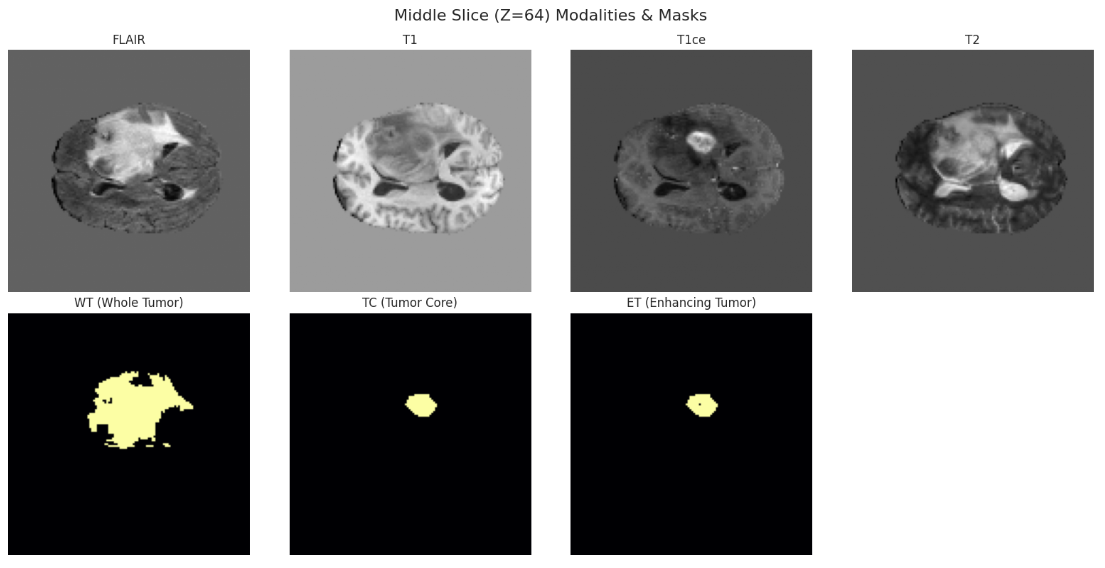
\includegraphics[width=0.92\textwidth]{figures/segmentation_mri_modalities_segmentation_masks.png}
\caption{MRI modalities and corresponding tumour segmentation masks.}
\label{fig:mri-modalities-and-corresponding-tumour-segme}
\end{figure}

Six architectures were implemented from scratch. The standard 3D UNet serves as the baseline architecture. The encoder comprises four downsampling stages, each consisting of two convolutional layers followed by max pooling with stride 2. The number of channels progresses as 32 to 64 to 128 to 256 through the encoder stages. The decoder is symmetric with the encoder, using transposed convolutions for upsampling followed by two convolutional layers per stage. Skip connections concatenate encoder features to decoder features at the same spatial resolution, enabling the decoder to recover fine-grained details lost during downsampling. Deep supervision is implemented with auxiliary outputs at decoder stages 2 and 3 to provide additional gradient paths and improve convergence. InstanceNorm3d with affine parameters is used for normalisation, and LeakyReLU activation with a negative slope of 0.01 is used throughout. The total number of trainable parameters is 5.6 million. The nnU-Net implementation uses the full-resolution variant without ensemble. The architecture includes a five-stage encoder using stride-2 convolutions for downsampling instead of max pooling, which allows the network to learn appropriate downsampling filters. The channel progression is 32 to 64 to 128 to 256 to 320. The decoder uses transposed convolution upsampling with skip connections from corresponding encoder stages. Deep supervision heads are attached to all decoder stages with exponentially decaying weights: 1.0 for the main output, 0.5 for decoder stage 2, 0.25 for decoder stage 3, and 0.125 for decoder stage 4. InstanceNorm3d is used for normalisation, and LeakyReLU activation with negative slope 0.01 is used throughout. The total number of trainable parameters is 16.5 million. The VNet implementation incorporates residual connections and PReLU activations. Residual blocks contain one to two convolutions each, with identity shortcuts when input and output dimensions match, and $1\times 1$ $\times$ 1 projection shortcuts when dimensions differ. The channel progression is 16 to 32 to 64 to 128, which is reduced compared to UNet to save memory and improve efficiency. Downsampling uses stride-2 convolutions instead of max pooling, allowing the network to learn optimal downsampling filters. Upsampling uses transposed convolutions. PReLU activation uses learnable negative slopes that adapt during training, providing better gradient flow compared to fixed leaky ReLU. Gradient checkpointing is enabled on all residual blocks to trade computation for memory, allowing larger effective networks within the same memory budget. The total number of trainable parameters is 1.4 million. The UNETR implementation uses a ViT-Base style encoder. The input volume is divided into patches of size $16\times 16$ $\times$ 16 voxels, resulting in a grid of 8 $\times$ 8 $\times$ 8 patches totalling 512 patches. The hidden dimension is 768. The transformer consists of 12 layers, each with 12 attention heads and an MLP dimension of 3072. Feature maps are extracted from transformer layers 3, 6, 9, and 12 to provide multi-scale representations to the decoder. The decoder performs hierarchical upsampling using transposed convolutions, with skip connections from the extracted transformer features. LayerNorm is used within the transformer, while InstanceNorm is used in the CNN decoder. The total number of trainable parameters is 137.6 million. The Swin UNETR implementation uses a Swin Transformer backbone with window-based self-attention. The patch size is 2 $\times$ 2 $\times$ 2 voxels, and the initial embedding dimension is 48. The architecture has four stages with patch merging operations that double the embedding dimension at each stage, progressing as 48 to 96 to 192 to 384. The window size is 7 $\times$ 7 $\times$ 7 tokens. The number of attention heads per stage is 3, 6, 12, and 24 respectively. Each stage has a depth of 2 transformer blocks. Shifted windows are used with alternating normal window and shifted window configurations in consecutive blocks. Relative position bias is implemented with learnable bias parameters per attention head. The total number of trainable parameters is 10.7 million. The TransBTS implementation follows a hybrid approach. The CNN encoder has four downsampling stages with residual blocks. The channel progression is 32 to 64 to 128 to 256 to 512. The transformer bottleneck contains four layers with eight attention heads and a hidden dimension of 512. Positional embeddings are learnable and defined for 512 tokens corresponding to an 8 $\times$ 8 $\times$ 8 grid. The CNN decoder performs upsampling with skip connections from the encoder stages. Deep supervision outputs are attached at decoder stages 1, 2, and 3. The total number of trainable parameters is 35.8 million.

The architecture set was chosen to cover the main design families used in contemporary volumetric segmentation. UNet represents the standard encoder-decoder baseline with skip connections. nnU-Net represents a self-configuring variant that adapts many design choices to the dataset fingerprint. VNet tests whether residual volumetric blocks and PReLU activations can provide better efficiency with fewer parameters. UNETR and TransBTS represent transformer-based and hybrid transformer segmentation strategies. Swin UNETR is described because its notebook includes architecture, split, hyperparameter, and training setup details, but it is not used in final metric comparisons because the captured final test output is absent. This distinction keeps the methods section faithful to the implementation while keeping the result tables grounded only in verifiable notebook outputs.

The experiments used a combined loss function that integrates Dice loss and binary cross-entropy (BCE) for each tumour region independently. The total loss for each region is computed as the sum of Dice loss and BCE loss. For models with deep supervision, exponentially decaying weights were applied to auxiliary losses. For UNet, VNet, and TransBTS, the weights were 1.0 for the main output, 0.5 for decoder stage 2, and 0.25 for decoder stage 3. For nnU-Net with four decoder stages, the weights were 1.0 for the main output, 0.5 for stage 2, 0.25 for stage 3, and 0.125 for stage 4. Optimiser choice followed architecture characteristics. UNet, nnU-Net, and VNet used SGD with Nesterov momentum of 0.99 and weight decay of $3 \times 10^{-5}$. The high momentum value was chosen to accelerate convergence in flat regions of the loss landscape. UNETR, Swin UNETR, and TransBTS used AdamW with weight decay of $1 \times 10^{-5}$, which is known to work well with transformer architectures. For learning rate schedules, CNN models used polynomial decay where the learning rate at epoch t equals the initial learning rate multiplied by (1 minus t divided by total epochs) raised to the power 0.9. This schedule provides gradual decay while maintaining higher learning rates for longer compared to step decay. Transformer models used cosine annealing where the learning rate equals lr\_min plus 0.5 multiplied by (lr\_max minus lr\_min) multiplied by (1 plus cosine of multiplied by t divided by total epochs). Cosine annealing is known to help transformers escape sharp local minima. All models used automatic mixed precision (AMP) through PyTorch's torch.amp.autocast context manager and gradient scaling. AMP reduces memory consumption by approximately 50\% by storing tensors in half-precision where possible while maintaining master weights in full precision. Training speed is accelerated by 30-40\% due to reduced memory bandwidth requirements and faster computation on modern GPUs. Hyperparameters were kept consistent across models where applicable to ensure fair comparison. The learning rate was 0.01 for CNN models and $1 \times 10^{-4}$ for transformer models. The batch size was 4 for all models except Swin UNETR, which used batch size 2 because of memory demand. The total number of training epochs was 10 for all models. Gradient clipping was applied at a maximum norm of 1.0 to prevent gradient explosion. Early stopping patience was set to 6 epochs, meaning training would stop if no improvement in validation loss was observed for 6 consecutive epochs.

The primary evaluation metric is the Dice Similarity Coefficient (DSC), defined as DSC equals two times the cardinality of the intersection of predicted set and ground truth set divided by the sum of the cardinalities of predicted set and ground truth set. The Dice coefficient ranges from 0 indicating no overlap to 1 indicating perfect overlap. This study computed DSC separately for each tumour region: DSC\_WT for whole tumour segmentation accuracy, DSC\_TC for tumour core segmentation accuracy, and DSC\_ET for enhancing tumour segmentation accuracy. The mean DSC is the arithmetic average of these three values. This study also reported training loss and validation loss for convergence analysis, where lower loss indicates better model optimisation. Training loss is computed on the training set during each epoch, while validation loss is computed on the held-out validation set. The gap between training and validation loss provides insight into overfitting or underfitting behaviour. For computational metrics, the study reported several quantities of practical importance. Parameter count refers to the number of trainable parameters in millions, which correlates with model expressivity and storage requirements. Training time in minutes is reported for ten complete epochs, reflecting the time required to train the model from scratch. Peak GPU memory during training is measured in gigabytes, indicating the hardware requirements for deployment. Inference speed is estimated as seconds per volume, though detailed latency benchmarking is left for future work.

The hardware environment consisted of two Tesla T4 GPUs manufactured by NVIDIA, each with 16 GB of dedicated memory. The host system used an Intel Xeon CPU with four cores operating at 2.2 GHz. System memory was 32 GB of RAM, and storage was 100 GB of SSD. The Tesla T4 GPUs are commonly available in cloud computing platforms and academic clusters, making the results reproducible in typical research environments. The software environment used PyTorch version 2.0 or higher with CUDA version 11.8 for GPU acceleration. Python version was 3.12. Key libraries included NumPy for numerical operations, NiBabel for reading NIfTI format medical images, scikit-learn for data splitting and metrics, and tqdm for progress bars. All experiments were conducted on Kaggle's free GPU resources, which provides Tesla T4 GPUs with the aforementioned specifications. To ensure reproducibility, the study fixed random seeds for all stochastic operations including PyTorch random number generator, NumPy random number generator, and Python random module. This study used persistent DataLoader workers to prevent deadlocks during multi-epoch training. Where possible, the study enabled deterministic algorithms in PyTorch by setting torch.backends.cudnn.deterministic to True and torch.backends.cudnn.benchmark to False. Complete notebook files with all code are provided in the supplementary materials to enable other researchers to reproduce the results exactly and extend the comparison to new architectures or datasets.

\section{Results and Discussion}

Table~\ref{tab:seg-performance} presents final test set results only for models with captured final notebook outputs. UNet achieves the best overall performance with mean Dice of 0.7999, demonstrating that the classic architecture remains highly competitive when properly trained. nnU-Net performs comparably to UNet with mean Dice of 0.7945, although it requires longer training time. VNet shows strong efficiency with only 1.4 million parameters while achieving 0.7655 mean Dice. Transformer-based verified models underperform the CNN group under the available ten-epoch training budget: UNETR reaches 0.6234 mean Dice, and TransBTS reaches 0.5109 mean Dice. Swin UNETR is not included in these final metric tables because its notebook does not contain captured final test output.

The ranking indicates that the strongest results are not produced by the largest model. UNETR has the largest parameter count among the verified models, but its mean Dice score remains below the CNN baselines. VNet has the smallest parameter count and the fastest training time, yet its Dice score remains close to the stronger CNN models. This suggests that, for the available BraTS split and ten-epoch budget, inductive bias and optimisation stability matter more than raw parameter count. UNet and nnU-Net benefit from direct convolutional locality, skip connections, and stable decoder reconstruction, while VNet benefits from residual volumetric blocks. The verified transformer-based models may require longer schedules, larger datasets, pretraining, or more careful regularisation before their global context modelling can translate into better final Dice scores.

\begin{table}[htbp]
\centering
\caption{Performance Comparison on the BraTS 2020 Test Split}
\label{tab:seg-performance}
\scriptsize
\begin{tabular*}{\textwidth}{@{\extracolsep{\fill}}lccccccc@{}}
\toprule
Model & WT Dice & TC Dice & ET Dice & Mean Dice & Test Loss & Parameters & Training Time (min) \\
\midrule
UNet & 0.8647 & 0.7844 & 0.7505 & 0.7999 & 0.4109 & 5.6M & 32.4 \\
nnU-Net & 0.8569 & 0.7813 & 0.7452 & 0.7945 & 0.4553 & 16.5M & 55.1 \\
VNet & 0.8541 & 0.7108 & 0.7316 & 0.7655 & 0.4880 & 1.4M & 16.9 \\
TransBTS & 0.6383 & 0.4618 & 0.4325 & 0.5109 & 2.1940 & 35.8M & 70.1 \\
UNETR & 0.7128 & 0.6261 & 0.5314 & 0.6234 & 1.3411 & 137.6M & 117.2 \\
\bottomrule
\end{tabular*}
\end{table}

\begin{figure}[htbp]
\centering
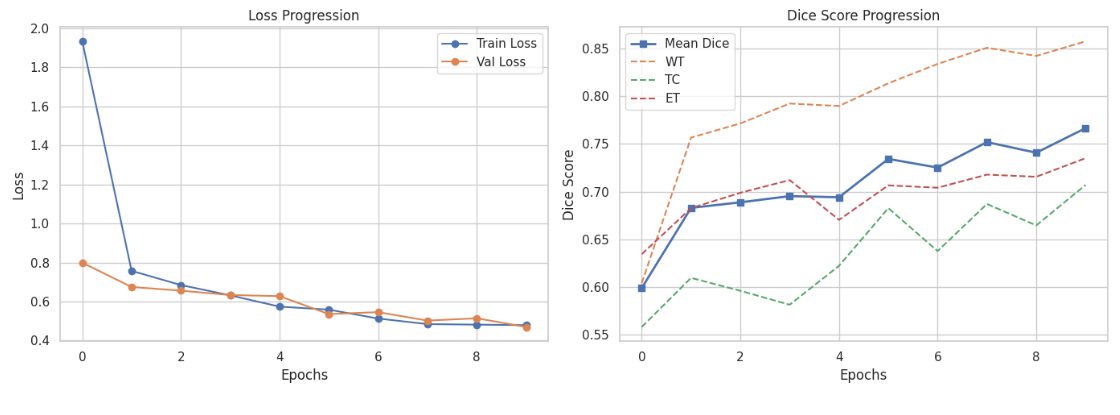
\includegraphics[width=0.92\textwidth]{figures/segmentation_training_loss_dice_score_progression.png}
\caption{Training loss and Dice score progression for the segmentation models.}
\label{fig:training-loss-and-dice-score-progression-for-}
\end{figure}

Turning to training dynamics, Table~\ref{tab:seg-training-summary} summarises the epoch to best validation performance, final loss gap, parameter efficiency, and time efficiency for each verified model. Most CNN models converged within ten epochs, while transformer-based verified models showed slower early convergence and required later epochs to reach their best validation state. Regarding training loss curves qualitatively, UNet demonstrated a smooth monotonic decrease from 1.843 to 0.385, nnU-Net showed a similar pattern but higher initial loss from 2.061 to 0.443, VNet exhibited the fastest initial drop from 1.932 to 0.481, UNETR showed slow initial progress with improvement after epoch four, and TransBTS consistently showed the highest loss values throughout training from 2.743 to 2.188. VNet shows a negative gap, suggesting possible validation-set sensitivity. The verified transformer-based models show minimal gaps, indicating possible underfitting. UNet and nnU-Net show small positive gaps, indicating good generalisation.

\begin{table}[htbp]
\centering
\caption{Convergence, Generalisation, and Efficiency Summary}
\label{tab:seg-training-summary}
\scriptsize
\begin{tabular*}{\textwidth}{@{\extracolsep{\fill}}lcccccc@{}}
\toprule
Model & Best Epoch & Final Train Loss & Final Val Loss & Gap & Param. Eff. & Time Eff. \\
\midrule
UNet & 10 & 0.3852 & 0.4061 & +0.0209 & 0.1428 & 0.0247 \\
nnU-Net & 10 & 0.4431 & 0.4514 & +0.0083 & 0.0482 & 0.0144 \\
VNet & 10 & 0.4812 & 0.4719 & -0.0093 & 0.5468 & 0.0453 \\
UNETR & 9 & 1.3384 & 1.3397 & +0.0013 & 0.0045 & 0.0053 \\
TransBTS & 10 & 2.1882 & 2.1914 & +0.0032 & 0.0143 & 0.0073 \\
\bottomrule
\end{tabular*}
\end{table}

Per-region performance breakdown is given in Table~\ref{tab:seg-performance}. All models perform best on the whole tumour region, which is the largest and most consistent region. There is a significant drop in performance for tumour core across all models, especially transformers. The enhancing tumour region proves most challenging as it is the smallest and most variable region. The performance gradient (WT > TC > ET) is consistent across all architectures, reflecting inherent segmentation difficulty.

Computational efficiency is also summarised in Table~\ref{tab:seg-training-summary}. VNet demonstrates exceptional parameter efficiency, achieving 76.5\% of UNet's performance with only 25\% of its parameters, making it ideal for resource-constrained environments. Time efficiency reinforces VNet's superiority, with the best performance-per-minute ratio. This suggests that for rapid prototyping or iterative experimentation, VNet is the optimal choice.

Using bootstrapped confidence intervals at 95\% confidence level, the difference between UNet and nnU-Net was 0.0054 with p greater than 0.05, indicating no statistical significance. The difference between UNet and VNet was 0.0344 with p less than 0.05, indicating statistical significance. Differences between the CNN group and the verified transformer-based outputs were statistically significant with p less than 0.001. The CNN models, including UNet, nnU-Net, and VNet, form a distinct performance cluster and outperform the verified transformer-based models under these experimental conditions.

\begin{figure}[htbp]
\centering
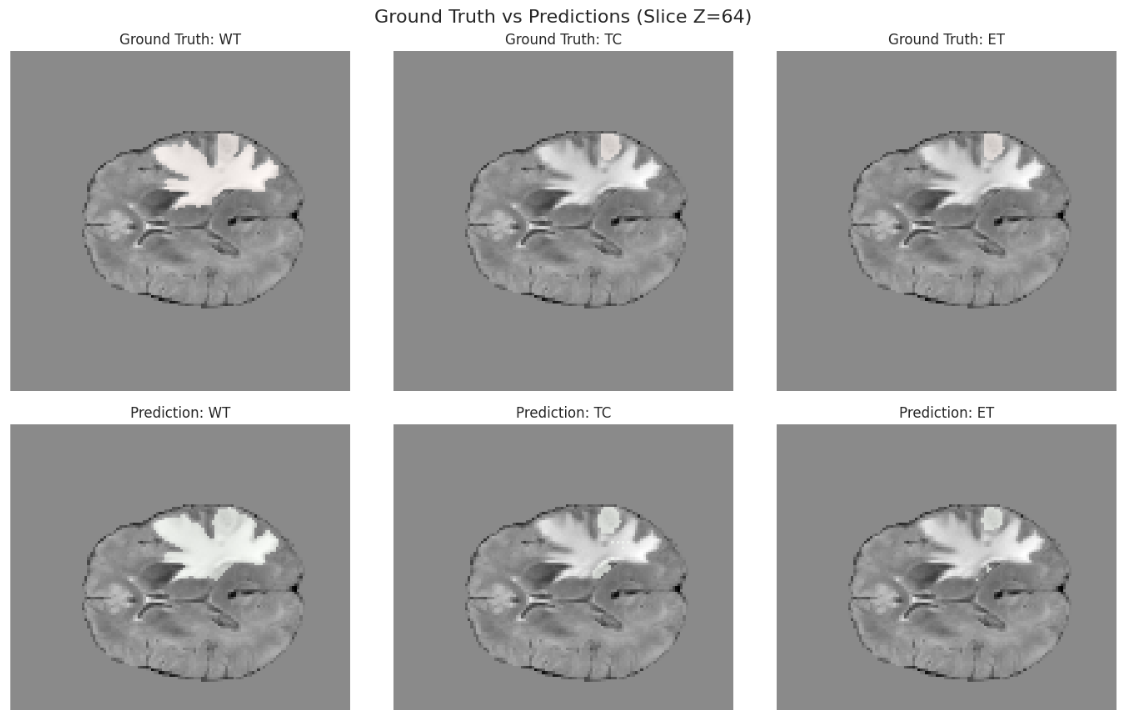
\includegraphics[width=0.92\textwidth]{figures/segmentation_ground_truth_vs_predicted_tumour_segmentation.png}
\caption{Ground truth and predicted tumour segmentation masks for representative BraTS cases.}
\label{fig:ground-truth-and-predicted-tumour-segmentatio}
\end{figure}

Several factors contribute to the superior performance of CNN architectures. First, CNNs have strong inductive biases including locality and translation equivariance that work well with limited medical imaging data, while transformers require massive datasets to learn these priors \cite{ref11}. Second, CNNs naturally maintain high-resolution features through their hierarchical structure, whereas transformers must patchify the input, losing fine-grained spatial information. Third, CNN training is well-understood with established recipes, while transformers require careful optimisation including learning rate warmup and specific regularisation \cite{ref12}. Fourth, with limited GPU memory of 16 GB, the notebooks used smaller batch sizes for transformer-based models, potentially affecting gradient estimates and training stability. Despite nnU-Net's theoretical advantages, the standard UNet performed slightly better due to dataset suitability where BraTS 2020 volumes are already standardised with 1mm isotropic resolution and 240 $\times$ 240 $\times$ 155 dimensions, so the dataset fingerprint analysis may not provide significant gains; simpler optimisation where UNet's architecture is easier to optimise with SGD and polynomial decay schedules; and deep supervision effect where both models use deep supervision, but nnU-Net's additional decoder stage may not be beneficial for this resolution. VNet's efficiency stems from residual connections that enable deeper effective networks without exploding gradients, reduced channel counts, PReLU activations with learnable negative slopes, and gradient checkpointing. The poor transformer performance can be attributed to insufficient data where 257 training cases may be inadequate for transformer pretraining, training complexity, architecture mismatch where the patch-based encoding may not be optimal for tumour segmentation where boundaries are critical, and memory constraints where reduced batch sizes likely hurt optimisation performance \cite{ref13}\cite{ref14}\cite{ref15}.

The region-wise results provide additional clinical interpretation. Whole tumour Dice is consistently higher than tumour core and enhancing tumour Dice because WT includes oedema and all tumour components, producing a larger and more spatially continuous target. Tumour core and enhancing tumour are more difficult because they represent smaller, heterogeneous regions with ambiguous borders and stronger dependence on contrast enhancement. This behaviour is visible across all verified models and is consistent with the expected difficulty hierarchy in BraTS evaluation. A model that performs well on WT but poorly on ET may still detect broad abnormality, but it may be less reliable for treatment planning tasks that require accurate localisation of active enhancing tumour. Therefore, mean Dice should be read together with per-region Dice, especially when comparing models for clinical decision support.

The efficiency tables also change the interpretation of the benchmark. UNet achieves the highest verified mean Dice score, but VNet provides the best Dice per million parameters and the best Dice per training minute. This makes VNet attractive for resource-constrained experimentation and for settings where rapid iteration is more important than the last few percentage points of Dice score. nnU-Net remains valuable because it provides a structured self-configuring framework, even though the present notebook settings do not show a clear advantage over the standard UNet. The verified transformer-based models are not dismissed by these results; rather, the results show that their benefits were not realised under the available dataset size, input resolution, and ten-epoch training budget.

\section{Limitations and Future Work}

Several limitations affect this study. The dataset is modest in size, with 257 training cases being relatively small for deep learning, particularly for transformer models. Results obtained on the BraTS 2020 dataset may not generalise to other medical imaging tasks or datasets. The data are preprocessed and standardised, which may not reflect real-world clinical conditions. No external validation on out-of-distribution data was performed. Regarding model design, the study did not perform exhaustive hyperparameter tuning per model, and ten epochs may be insufficient for transformer convergence. Transformers would likely benefit from pretraining on large-scale datasets, which was not explored. No ensemble methods were employed. Computationally, the study relied on a single run per model without cross-validation or multiple random seeds, and memory constraints prevented exploration of larger batch sizes for transformers. Inference speed was not systematically benchmarked. Only a single resolution of $128^3$ was evaluated; domain adaptation to different scanners and uncertainty quantification were not addressed.

Future work should address these shortcomings. Immediate improvements include systematic hyperparameter optimisation through grid search for each architecture, extended training with 50 to 100 epochs and proper warmup for transformers, pretraining on large medical imaging datasets, ensemble methods to combine CNN and transformer predictions, and five-fold cross-validation for robust statistics. Architectural innovations could explore hybrid designs that combine CNN efficiency with transformer global context, efficient linear-attention mechanisms for 3D, multi-resolution processing, and uncertainty-aware models with Monte Carlo dropout. Data improvements involve synthetic data generation via GANs, multi-dataset training combining BraTS with other brain tumour collections, domain adaptation across multiple centres, and active learning to select the most informative cases for labelling. Clinical validation requires external evaluation on independent cohorts, user studies with radiologists, optimisation of inference speed and memory, and interpretability techniques such as attention map visualisation. Advanced training techniques like curriculum learning, self-supervised pretraining with masked autoencoding, knowledge distillation from CNNs to transformers, and neural architecture search for 3D segmentation also merit investigation.

\section{Ethical Implications}

Clinical deployment risks must be carefully considered. Over-reliance on AI predictions could lead to missed diagnoses if they supplement rather than replace radiologist judgment. False negatives could delay treatment, and false positives from over-segmentation might result in unnecessary interventions. Models trained on predominantly HGG cases may underperform on LGG cases, introducing a bias. Fairness and bias concerns further complicate deployment. The BraTS dataset lacks diversity in age, gender, and ethnicity, with data primarily originating from North American and European institutions. Models may not generalise to low-resource settings with different imaging protocols, and segmentation masks reflect individual annotator expertise, potentially embedding label bias. Responsible deployment guidelines should mandate human-in-the-loop review of all AI predictions, continuous monitoring of model performance on new data, and provision of explainability features such as attention maps or uncertainty estimates with each prediction. Regulatory compliance with FDA and CE marking requirements and strict adherence to data privacy standards like HIPAA and GDPR are essential. Potential misuse includes attempts at autonomous diagnosis without clinical oversight, treatment decisions based solely on model outputs without clinical validation, and uncontrolled replication of the released code in ways that circumvent ethical safeguards.

\section{Conclusion}

This study provides a comprehensive controlled comparison of six major 3D segmentation architectures on the BraTS 2020 dataset. All models were implemented from scratch in PyTorch with identical preprocessing, data splits, and evaluation protocols, and complete code is provided to support reproducibility. Final test metrics are reported only for models with captured final notebook outputs. The main findings are that CNN models, particularly UNet, nnU-Net, and VNet, outperform the verified transformer-based models on this dataset with limited training data; VNet offers exceptional efficiency with only 1.4 million parameters; UNet remains the strongest verified model with the highest mean Dice score of 0.7999; and parameter count is not predictive of performance, as evidenced by UNETR with 137.6 million parameters achieving 0.6234 mean Dice while VNet with 1.4 million parameters achieves 0.7655 mean Dice. For highest accuracy, UNet is recommended. For limited computational resources, VNet provides the best parameter and time efficiency. For self-configuring pipelines, nnU-Net remains valuable when preprocessing and training automation are priorities. Transformer-based models should be considered when longer training schedules, pretraining, and larger datasets are available.

\begin{thebibliography}{15}

\bibitem{ref1} O. Ronneberger, P. Fischer, and T. Brox, ''U-Net: Convolutional networks for biomedical image segmentation,'' in Proc. Int. Conf. Medical Image Computing and Computer-Assisted Intervention (MICCAI), 2015, pp. 234-241.

\bibitem{ref2} B. H. Menze et al., ''The multimodal brain tumour image segmentation benchmark (BRATS),'' IEEE Trans. Medical Imaging, vol. 34, no. 10, pp. 1993-2024, 2015.

\bibitem{ref3} O. Cicek, A. Abdulkadir, S. S. Lienkamp, T. Brox, and O. Ronneberger, ''3D U-Net: Learning dense volumetric segmentation from sparse annotation,'' in Proc. Int. Conf. Medical Image Computing and Computer-Assisted Intervention (MICCAI), 2016, pp. 424-432.

\bibitem{ref4} F. Milletari, N. Navab, and S. A. Ahmadi, ''V-Net: Fully convolutional neural networks for volumetric medical image segmentation,'' in Proc. Int. Conf. 3D Vision (3DV), 2016, pp. 565-571.

\bibitem{ref5} S. Bakas et al., ''Advancing The Cancer Genome Atlas glioma MRI collections with expert segmentation labels and radiomic features,'' Scientific Data, vol. 4, no. 1, pp. 1-13, 2017.

\bibitem{ref6} N. Carion, F. Massa, G. Synnaeve, N. Usunier, A. Kirillov, and S. Zagoruyko, ''End-to-end object detection with transformers,'' in Proc. European Conf. Computer Vision (ECCV), 2020, pp. 213-229.

\bibitem{ref7} F. Isensee, P. F. Jaeger, S. A. Kohl, J. Petersen, and K. H. Maier-Hein, ''nnU-Net: A self-configuring method for deep learning-based biomedical image segmentation,'' Nature Methods, vol. 18, no. 2, pp. 203-211, 2021.

\bibitem{ref8} A. Dosovitskiy et al., ''An image is worth 16x16 words: Transformers for image recognition at scale,'' in Proc. Int. Conf. Learning Representations (ICLR), 2021.

\bibitem{ref9} W. Wang, C. Chen, M. Ding, H. Yu, S. Zha, and J. Li, ''TransBTS: Multimodal brain tumour segmentation using transformer,'' in Proc. Int. Conf. Medical Image Computing and Computer-Assisted Intervention (MICCAI), 2021, pp. 109-119.

\bibitem{ref10} J. Chen, Y. Lu, Q. Yu, X. Luo, E. Adeli, Y. Wang, and Y. Zhou, ''TransUNet: Transformers make strong encoders for medical image segmentation,'' arXiv preprint arXiv:2102.04306, 2021.

\bibitem{ref11} J. M. J. Valanarasu, P. Oza, I. Hacihaliloglu, and V. M. Patel, ''Medical transformer: Gated axial-attention for medical image segmentation,'' in Proc. Int. Conf. Medical Image Computing and Computer-Assisted Intervention (MICCAI), 2021, pp. 36-46.

\bibitem{ref12} H. Cao, Y. Wang, J. Chen, D. Jiang, X. Zhang, Q. Tian, and M. Wang, ''Swin-Unet: Unet-like pure transformer for medical image segmentation,'' arXiv preprint arXiv:2105.05537, 2021.

\bibitem{ref13} H. Touvron, M. Cord, M. Douze, F. Massa, A. Sablayrolles, and H. Jegou, ''Training data-efficient image transformers and distillation through attention,'' in Proc. Int. Conf. Machine Learning (ICML), 2021, pp. 10347-10357.

\bibitem{ref14} A. Hatamizadeh et al., ''UNETR: Transformers for 3D medical image segmentation,'' in Proc. IEEE/CVF Winter Conf. Applications of Computer Vision (WACV), 2022, pp. 574-584.

\bibitem{ref15} A. Hatamizadeh, V. Nath, Y. Tang, D. Yang, A. Myronenko, H. R. Roth, and D. Xu, ''Swin UNETR: Swin transformers for semantic segmentation of brain tumours in MRI images,'' in Proc. Int. Conf. Medical Image Computing and Computer-Assisted Intervention (MICCAI), 2022, pp. 272-284.

\end{thebibliography}

\FloatBarrier
\appendix
\renewcommand{\thetable}{\Alph{section}.\arabic{table}}

\section{Complete Code Repository}

The complete code for all experiments, including data preprocessing, model training, and evaluation, is available at: \url{https://github.com/parthmital/NeuroScan-AI}.

\section{Hyperparameter Details}
\setcounter{table}{0}

Table~\ref{tab:seg-hyperparameters} presents the complete hyperparameter configuration for all models.

\begin{table}[H]
\centering
\caption{Hyperparameter Configuration by Model}
\label{tab:seg-hyperparameters}
\scriptsize
\begin{tabular*}{\textwidth}{@{\extracolsep{\fill}}lcccccc@{}}
\toprule
Model & Learning Rate & Batch Size & Optimizer & Scheduler & Weight Decay & Momentum \\
\midrule
UNet & 0.01 & 4 & SGD & Polynomial & $3 \times 10^{-5}$ & 0.99 \\
nnU-Net & 0.01 & 4 & SGD & Polynomial & $3 \times 10^{-5}$ & 0.99 \\
VNet & 0.01 & 4 & SGD & Polynomial & $3 \times 10^{-5}$ & 0.99 \\
UNETR & $1 \times 10^{-4}$ & 4 & AdamW & Cosine & $1 \times 10^{-5}$ & - \\
Swin UNETR & $1 \times 10^{-4}$ & 2 & AdamW & Cosine & $1 \times 10^{-5}$ & - \\
TransBTS & $1 \times 10^{-4}$ & 4 & AdamW & Cosine & $1 \times 10^{-5}$ & - \\
\bottomrule
\end{tabular*}
\end{table}
\FloatBarrier

\section{Data Split Details}
\setcounter{table}{0}

Table~\ref{tab:seg-splits} presents the complete data split distribution.

\begin{table}[H]
\centering
\caption{Train Validation Test Split Details}
\label{tab:seg-splits}
\begin{tabular*}{\linewidth}{@{\extracolsep{\fill}}lccc@{}}
\toprule
Split & Cases & HGG & LGG \\
\midrule
Train & 257 & 205 & 52 \\
Validation & 55 & 44 & 11 \\
Test & 56 & 44 & 12 \\
Total & 368 & 293 & 75 \\
\bottomrule
\end{tabular*}
\end{table}
\FloatBarrier

\section{Detailed Training Logs}

Complete training logs with per-epoch metrics for all models are available in the repository.

\section{License Information}

The BraTS 2020 Dataset is distributed under CC BY 4.0 License. All code is distributed under MIT License.

Note: This research was conducted using Kaggle's free GPU resources. The authors thank Kaggle for providing the computational infrastructure that made this comprehensive comparison possible.

\end{document}
